\documentclass[crop,tikz,border=10]{standalone}

\usepackage{amsmath, amssymb}
\usetikzlibrary{calc}
\usetikzlibrary{matrix}


\newcommand{\rr}{0.7}
\newcommand{\qq}{0.75}
\begin{document}
    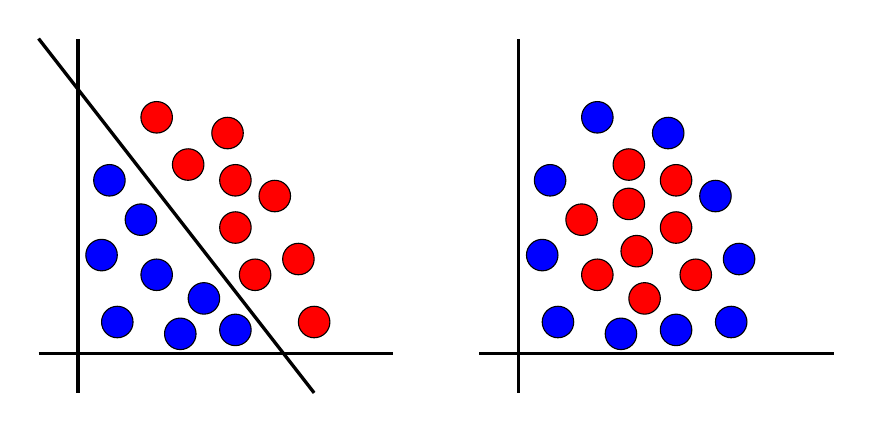
\begin{tikzpicture}
        \matrix[column sep=3em] {
            \draw[very thick] (0, -0.5) -- (0, 4);
            \draw[very thick] (-0.5, 0) -- (4, 0);

            \draw[very thick] (-0.5, 4) -- (3, -0.5);
            \draw[fill=blue] (1, 1) circle (0.2);
            \draw[fill=blue] (0.5, 0.4) circle (0.2);
            \draw[fill=blue] (2, 0.3) circle (0.2);
            \draw[fill=blue] (1.3, 0.25) circle (0.2);
            \draw[fill=blue] (0.4, 2.2) circle (0.2);
            \draw[fill=blue] (0.3, 1.25) circle (0.2);
            \draw[fill=blue] (0.8, 1.7) circle (0.2);
            \draw[fill=blue] (1.6, 0.7) circle (0.2);

            \draw[fill=red] (2.25, 1) circle (0.2);
            \draw[fill=red] (3, 0.4) circle (0.2);
            \draw[fill=red] (2, 1.6) circle (0.2);
            \draw[fill=red] (2.8, 1.2) circle (0.2);
            \draw[fill=red] (2.5, 2) circle (0.2);
            \draw[fill=red] (1.4, 2.4) circle (0.2);
            \draw[fill=red] (2, 2.2) circle (0.2);
            \draw[fill=red] (1.9, 2.8) circle (0.2);
            \draw[fill=red] (1, 3) circle (0.2);
            &
            \draw[very thick] (0, -0.5) -- (0, 4);
            \draw[very thick] (-0.5, 0) -- (4, 0);

            \draw[fill=red] (1, 1) circle (0.2);
            \draw[fill=blue] (0.5, 0.4) circle (0.2);
            \draw[fill=blue] (2, 0.3) circle (0.2);
            \draw[fill=blue] (1.3, 0.25) circle (0.2);
            \draw[fill=blue] (0.4, 2.2) circle (0.2);
            \draw[fill=blue] (0.3, 1.25) circle (0.2);
            \draw[fill=red] (0.8, 1.7) circle (0.2);
            \draw[fill=red] (1.6, 0.7) circle (0.2);
            \draw[fill=red] (1.5, 1.3) circle (0.2);
            \draw[fill=red] (1.4, 1.9) circle (0.2);

            \draw[fill=red] (2.25, 1) circle (0.2);
            \draw[fill=blue] (2.7, 0.4) circle (0.2);
            \draw[fill=red] (2, 1.6) circle (0.2);
            \draw[fill=blue] (2.8, 1.2) circle (0.2);
            \draw[fill=blue] (2.5, 2) circle (0.2);
            \draw[fill=red] (1.4, 2.4) circle (0.2);
            \draw[fill=red] (2, 2.2) circle (0.2);
            \draw[fill=blue] (1.9, 2.8) circle (0.2);
            \draw[fill=blue] (1, 3) circle (0.2);
            \\
        };
    \end{tikzpicture}
\end{document}